\documentclass{beamer}
\usepackage[french]{babel}
\usepackage{graphicx}
\usepackage{listings}

\usetheme{Rochester}
\usecolortheme{dolphin}

\title{SoftDesk: mise en place d'une API REST sécurisée}
\subtitle{Openclassrooms, parcours python, projet 10}
\author{Bérenger Ossété Gombé}

\begin{document}

\begin{frame}
  \maketitle
\end{frame}

\begin{frame}{Table des matières}
  \tableofcontents
\end{frame}

\section{Introduction}

\begin{frame}{Introduction}
  \begin{block}{Bérenger Ossété Gombé}
    \begin{itemize}
    \item Bac scientifique en 2013
    \item Maîtrise en informatique (génie logiciel) en 2017
    \item Reconversion web chez Openclassrooms depuis janvier 2022
    \end{itemize}
  \end{block}
\end{frame}

\begin{frame}{Créez une API sécurisée RESTful en utilisant Django REST}
  \begin{block}{Projet 10: parcours python}
    \begin{itemize}
    \item Documenter une application
    \item Créer une API RESTful
    \item Sécuriser une API (OWASP et RGPD)
    \end{itemize}
  \end{block}
\end{frame}

\begin{frame}{Contexte du projet}
  \begin{center}
    
\includegraphics[scale=0.3]{images/logo.png}
  \end{center}
  
  \begin{block}{SoftDesk}
    \begin{itemize}
    \item Société d'édition de logiciels.
    \item Veut développez un \textbf{système de suivi de problèmes}.
    \item Nous sommes ingénieur \textit{backend} sur cette
      application.
    \end{itemize}
  \end{block}
\end{frame}

\section{Exigences}

\begin{frame}{Exigences}
  \begin{block}{Exigences fonctionnelles}
    \begin{itemize}
    \item En tant qu'utilisateur nous pouvons \textbf{nous authentifier}.
    \item En tant qu'utilisateur nous pouvons \textbf{manipuler des projets}.
    \item En tant que contributeur d'un projet nous pouvons
      \textbf{manipuler les problèmes} qui lui sont liés.
    \item En tant que contributeur d'un projet nous pouvons
      \textbf{commenter les problèmes} qui lui sont liés.
    \item En tant qu'auteur d'un problème, d'un projet, ou d'un
      commentaire nous pouvons l'\textbf{actualiser et le supprimer}.
    \item En tant qu'auteur d'un projet nous pouvons \textbf{ajouter
      ou supprimer un collaborateur}.
    \end{itemize}
  \end{block}
\end{frame}

\begin{frame}{Différents droits d'accès}
  \begin{block}{Droits d'accès}
    \begin{center}
      \small
      \begin{tabular}{|r|c|c|c|}
        \hline
        & Auteur & Collaborateur & Utilisateur \\
        \hline
        créer un projet & \checkmark & \checkmark & \checkmark \\
        consulter un projet & \checkmark & \checkmark & - \\
        éditer un projet & \checkmark & - & - \\
        supprimer un projet & \checkmark & - & - \\
        \hline
        créer un problème & \checkmark & \checkmark & - \\
        consulter un problème & \checkmark & \checkmark & - \\
        éditer un problème & \checkmark & - & - \\
        supprimer un problème & \checkmark & - & - \\
        \hline
        créer un commentaire & \checkmark & \checkmark & - \\
        consulter un commentaire & \checkmark & \checkmark & - \\
        éditer un commentaire & \checkmark & - & - \\
        supprimer un commentaire & \checkmark & - & - \\
        
        \hline
      \end{tabular}
    \end{center}
  \end{block}
\end{frame}

\section{API REST}

\begin{frame}{API REST}
  \begin{block}{Les ressources}
    \begin{center}
      \begin{tabular}{|r|l|}
        \hline
        Nom & URI \\
        \hline
        \hline
        Projet & $/projects/$ \\
        Collaborateur & $/projects/\{id\}/users/$ \\
        Problème & $/projects/\{id\}/issues/$ \\
        Commentaires & $/projects/\{id\}/issues/\{id\}/comments/$ \\
        \hline
      \end{tabular}
    \end{center}
  \end{block}

  \begin{block}{Actions}
    \begin{center}
      \begin{tabular}{|r|l|}
        \hline
        Création & POST \\
        \hline
        Accès & GET \\
        \hline
        Mise à jour & PUT \\
        \hline
        Suppression & DELETE \\
        \hline
      \end{tabular}
    \end{center}
  \end{block}
\end{frame}

\section{Documentation}

\begin{frame}{Documentation}  
\end{frame}

\begin{frame}{Pourquoi documenter ?}
  \begin{block}{Plusieurs raisons de maintenir la documentation d'un projet}
    \begin{itemize}
    \item Le projet peut être co-développé par de nombreux contributeurs.
    \item Centralise les informations importantes.
    \item Les contributeurs du projet peuvent être amenés à changer:
    \item Facilite la formation des nouveaux développeurs.
    \item Cela peut permettre une traçabilité des fonctionnalités.
    \end{itemize}
  \end{block}
\end{frame}

\begin{frame}{Quoi documenter ?}
  \begin{block}{Tout au long du cycle de vie du logiciel}
    \begin{itemize}
    \item Les exigences (cahier des charges)
    \item Le développement (dans le code source et la documentation externe)
    \item Les tests (plan de test, stratégie de test, ...)
    \item Les analyses et audits
    \item Le manuel pour utilisateurs ou développeurs
    \end{itemize}
  \end{block}
\end{frame}

\begin{frame}{Documentation et développement}
  \begin{block}{\textit{Documentation Driven Development}}
    \begin{itemize}
    \item Mise en place d'une documentation \textbf{avant} l'implémentation.
    \end{itemize}
  \end{block}

  
  \begin{block}{Où et comment documenter l'API ?}
    \begin{itemize}
    \item Utilisation de \textsf{sphinx}
    \item Utilisation de \textsf{Postman}
    \item Autre possibilité: \textit{github} propose des pages web par projets ainsi qu'un wiki.
    \end{itemize}
  \end{block}  
\end{frame}

\begin{frame}{Documenter le code}
  \begin{block}{Sphinx}
    \begin{itemize}
    \item Utilisée par \textsf{read the docs}
    \item Permet de créer une documentation à partir de fichiers
      \textsf{reStructuredText}.
    \end{itemize}
  \end{block}  
\end{frame}

\begin{frame}[fragile]{Documentation: Sphinx}
  \tiny
  \begin{center}
    \begin{figure}
      \begin{lstlisting}
        This is a Title
        ===============
        That has a paragraph about a main subject and is set when the '='
        is at least the same length of the title itself.

        Subject Subtitle
        ----------------
        Subtitles are set with '-' and are required to have the same length
        of the subtitle itself, just like titles.

        Lists can be unnumbered like:

        * Item Foo
        * Item Bar

        Or automatically numbered:

        #. Item 1
        #. Item 2

        Inline Markup
        -------------
        Words can have *emphasis in italics* or be **bold** and you can define
        code samples with back quotes, like when you talk about a command: ``sudo``
        gives you super user powers!
      \end{lstlisting}      
      \caption{Exemple de document rédigé \textit{via} la syntaxe \textsf{reStructuredText}}      
    \end{figure}
  \end{center}
\end{frame}

\section{Sécurité}

\begin{frame}{Sécurité}  
\end{frame}

\begin{frame}{Enjeux de la sécurité}

  \begin{block}{Tout est une question de \underline{risques}}
    Risque = un impact x probabilité d'occurrence
  \end{block}

  \begin{block}{Rédaction d'un modèle de menaces (\textit{threats modelling})}
    Quatre questions à se poser\footnote{\url{https://owasp.org/www-community/Threat_Modeling}}:
    \begin{itemize}
    \item Sur quoi travaillons-nous ?
    \item Qu'est-ce qu'il pourrait arriver de mauvais ?
    \item Quoi faire si cela arrive ?
    \item Avons-nous fait du bon travail ?
    \end{itemize}
  \end{block}
\end{frame}

\begin{frame}{OWASP}
  \begin{block}{Top 10}
    \begin{itemize}
    \item \textit{Open Web Application Security Project}.
    \item Propose (entre autres) un classement des 10 risques de
      sécurités les plus critiques.
    \end{itemize}
  \end{block}
\end{frame}

\begin{frame}{OWASP 2021}
  \begin{block}{Le top 10 des menaces de sécurité}
    Version 2021 du Top 10 OWASP\footnote{\url{https://owasp.org/Top10/fr/}}:
    \begin{enumerate}
    \item Contrôles d'accès défaillants.
    \item Défaillances cryptographiques.
    \item Injections.
    \item Conception non-sécurisée.
    \item Mauvaise configuration de sécurité.
    \item Composants vulnérables et obsolètes.
    \item Identification et authentification de mauvaise qualité.
    \item Manque d'intégrité des données et du logiciel.
    \item Carence des systèmes de contrôle et de journalisation.
    \item Falisification des requêtes côté serveur.
    \end{enumerate}
  \end{block}
\end{frame}

\begin{frame}{Comparaison avec l'OWASP 2017}
  \begin{center}
    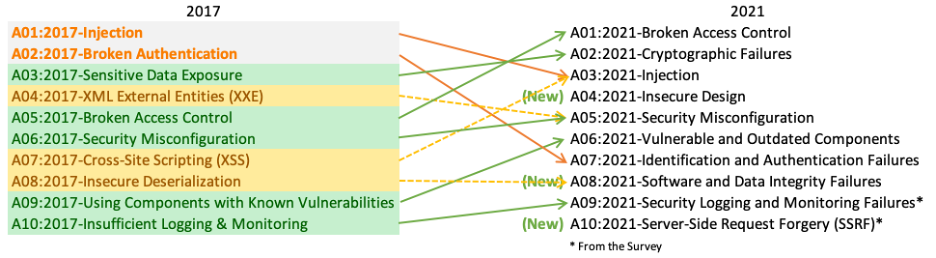
\includegraphics[scale=0.7]{images/owasp_mapping.png}
  \end{center}
\end{frame}

\begin{frame}{Sécurité mise en place par Django}
  \begin{block}{Protection contre les attaques XSS}
    Le système de \textit{template} de django échappe certains
    caractères \textbf{mais} ne protège pas contre toutes les
    attaques XSS\footnote{\url{https://docs.djangoproject.com/fr/4.1/topics/security/}}.
    \begin{itemize}
    \item \textit{via} du code HTML et JS dans les variables
    \item \textit{via} du code HTML en base de données
    \end{itemize}
  \end{block}

  \begin{block}{Protection contre les attaques CSRF}
    Protection par le \textit{middleware} \textsf{CSRFViewMiddleware}.
    Cependant il faut être prudent lors de l'utilisation du décorateur
    \textsf{csrf\_exempt}.
  \end{block}

  \begin{block}{Protection contre les injections SQL}
    À moins que l'on n'écrive des requêtes en SQL brutes, le système
    de paramétrisation apporte une protection aux injections SQL.
  \end{block}
\end{frame}

\begin{frame}{Sécurité et configuration de Django}
  \begin{block}{Autres protections\footnote{\url{https://docs.djangoproject.com/fr/4.1/topics/security/}}}
    \begin{itemize}
    \item Détournement de clic (\textit{via} les \textit{frames} HTML).
    \item SSL et HTTPS.
    \item Validation de l'entête HTTP ``Host''.
    \item Sécurité des sessions.
    \item ...
    \end{itemize}
  \end{block}

  \begin{block}{Mise en production}
    Django propose une commande permettant de vérifier la sécurité
    d'une application web avant sa mise en production.
    
    \textsf{./manage.py check --deploy}
  \end{block}
\end{frame}

\begin{frame}{Renforcer la sécurité}
  \begin{block}{Sécurités supplémentaires}
    \begin{itemize}
    \item Authentification par nom d'utilisateur et mot de passe:
      \begin{itemize}
      \item Vérification de la sécurité du mot de passe.
      \end{itemize}
    \item Mise en place d'un système de rôles:
      \begin{itemize}
      \item Administrateur
      \item Auteur d'un projet, d'un problème ou d'un commentaire
      \item Collaborateur
      \item Utilisateur
      \end{itemize}
    \end{itemize}
  \end{block}
\end{frame}

\begin{frame}{Tester la sécurité de l'API}
  \begin{block}{Différents types de tests}
    \begin{itemize}
    \item \textit{Scan} de vulnérabilités
    \item Tests de pénétrations
    \item Audits de sécurité
    \item ...
    \end{itemize}

    Comment tester la sécurité de l'API ?
  \end{block}

  \begin{block}{\textit{Via} Django}
    Il est possible d'utiliser les tests Django pour vérifier la
    sécurité du système développé. Il existe différents niveaux de
    tests: ici nous parlons de tests non fonctionnels d'acceptations
    et non pas de tests fonctionnels unitaires ($\rightarrow$ en
    complément, non pas à la place).
  \end{block}
\end{frame}


\begin{frame}{Respect de la RGPD}
  \begin{block}{Quelques points importants pour le respect de la RGPD}
    \begin{itemize}
    \item Les données personnelles sont chiffrées dans la base de données.
    \item Un utilisateur connecté peut actualiser ou supprimer toutes
      les ressources dont il est l'auteur.
    \item Les données personnelles stockées en base de données sont réduites.
    \item Après publication, il doit être possible pour un utilisateur de
      demander la suppression de toutes ses données personnelles.
    \item $\rightarrow$ C'est une question de droit, la consultation
      d'un juriste est souvent conseillée.
    \end{itemize}

    $\rightarrow$ Voir \url{https://www.economie.gouv.fr/entreprises/reglement-general-sur-protection-des-donnees-rgpd}
  \end{block}
\end{frame}


\section{Démonstration}

\begin{frame}{Démonstration avec POSTMAN}
  \begin{block}{Démonstration}
    \begin{itemize}
    \item Démonstration de l'API.
    \item Démonstration de la documentation.
    \end{itemize}
  \end{block}
\end{frame}

\section{Développement}

\begin{frame}{Développement}  
\end{frame}

\begin{frame}{Vue d'ensemble}
  \begin{block}{Applications}
    \begin{itemize}
    \item \textsf{authentication}: pour gérer les utilisateurs et
      l'authentification.
    \item \textsf{project}: pour gérer les projets et ce qui tournent
      autour.
    \end{itemize}
  \end{block}
\end{frame}

\begin{frame}[fragile]{L'authentification}
  \begin{itemize}
  \item Authentification par jeton JWT.
  \item Utilisation de la bibliothèque
    \textsf{djangorestframework-simplejwt}.
  \item Fournit une vue toute faite \textsf{TokenObtainPairView}.
  \end{itemize}

  \begin{center}
    \tiny
    \begin{lstlisting}[language=python]
      ...
      from rest_framework_simplejwt.views import TokenObtainPairView
      
      urlpatterns = [
          ...
          path('login/', TokenObtainPairView.as_view(), name='login')    
      ]
    \end{lstlisting}
  \end{center}
\end{frame}

\begin{frame}{Les rôles}
  \begin{block}{Plusieurs rôles possibles}
    \begin{itemize}
    \item Collaborateur d'un projet:
      \begin{itemize}
      \item Contributeur (\textit{contributor})
      \item Responsable (\textit{supervisor})
      \item Auteur (\textit{author})
      \end{itemize}
    \item Un utilisateur peut avoir plusieurs rôles !
    \end{itemize}
  \end{block}
\end{frame}

\begin{frame}[fragile]{Modèle d'un collaborateur}
  \begin{center}
    \tiny
    \begin{lstlisting}[language=python]
    class Collaborator(models.Model):
      SUPERVISOR_ROLE = 'SUPERVISOR'
      CONTRIBUTOR_ROLE = 'CONTRIBUTOR'
      AUTHOR_ROLE = 'AUTHOR'
      
      ROLES = [
        (SUPERVISOR_ROLE, 'supervisor'),
        (CONTRIBUTOR_ROLE, 'contributor'),
        (AUTHOR_ROLE, 'author')
      ]
      
      user = models.ForeignKey(User, on_delete=models.CASCADE)
      project = models.ForeignKey(Project, on_delete=models.CASCADE)
      role = models.CharField(max_length=256, choices=ROLES)
    \end{lstlisting}
  \end{center}
\end{frame}

\begin{frame}[fragile]{Les projets}
  \begin{block}{Un projet c'est:}
    \begin{itemize}
    \item Un titre.
    \item Une description.
    \item Un type: ANDROID, IOS, FRONTEND ou BACKEND.
    \end{itemize}
  \end{block}

  \begin{center}
    \tiny
    \begin{lstlisting}[language=python]
  class Project(models.Model):
    ANDROID_TYPE = 'ANDROID'
    IOS_TYPE = 'IOS'
    BACKEND_TYPE = 'BACKEND'
    FRONTEND_TYPE = 'FRONTEND'
    
    TYPES = [
        (ANDROID_TYPE, 'Android'),
        (IOS_TYPE, 'IOS'),
        (BACKEND_TYPE, 'Back-end'),
        (FRONTEND_TYPE, 'Front-End')
    ]
    
    title = models.CharField(max_length=256)
    description = models.CharField(max_length=4096)
    type = models.CharField(max_length=64, choices=TYPES)
    \end{lstlisting}
  \end{center}
\end{frame}

\begin{frame}[fragile]{Modèle d'un problème}
  \begin{center}
    \tiny
    \begin{lstlisting}[language=python]
      class Issue(models.Model):
        # ...
      
        title = models.CharField(max_length=256)
        description = models.CharField(max_length=4096)
        tag = models.CharField(max_length=128, choices=TAGS)
        priority = models.IntegerField()
        status = models.CharField(max_length=128, choices=STATUS)
        project = models.ForeignKey(Project, on_delete=models.CASCADE)
        author = models.ForeignKey(
            User,
            on_delete=models.CASCADE,
            related_name='author'
        )
        assignee = models.ForeignKey(
            User,
            on_delete=models.CASCADE,
            related_name='assignee'
        )
        created = models.DateTimeField(auto_now=True)
    \end{lstlisting}
  \end{center}
\end{frame}

\begin{frame}[fragile]{Tags et status}
  \begin{center}
    \tiny
    \begin{lstlisting}[language=python]
      class Issue(models.Model):
        BUG_TAG = 'BUG'
        IMPROVEMENT_TAG = 'IMPROVEMENT'
        TASK_TAG = 'TASK'
        
        TAGS = [
            (BUG_TAG, 'bug'),
            (IMPROVEMENT_TAG, 'improvement'),
            (TASK_TAG, 'task')
        ]
        
        OPEN_STATUS = 'OPEN'
        CLOSED_STATUS = 'CLOSED'
        
        STATUS = [
            (OPEN_STATUS, 'open'),
            (CLOSED_STATUS, 'closed')
        ]

        # ...
    \end{lstlisting}
  \end{center}
\end{frame}

\begin{frame}[fragile]{Modèle d'un commentaire}
  \begin{center}
    \tiny
    \begin{lstlisting}[language=python]
      class Comment(models.Model):
        description = models.CharField(max_length=4096)
        author = models.ForeignKey(User, on_delete=models.CASCADE)
        issue = models.ForeignKey(Issue, on_delete=models.CASCADE)
        created = models.DateTimeField(auto_now=True)
    \end{lstlisting}
  \end{center}
\end{frame}


\begin{frame}[fragile]{Sérialisation des modèles}
  \begin{block}{Motivation}
    \begin{itemize}
    \item Permet de passer d'une classe python au format JSON.
    \item Utilisation de la classe \textsf{ModelSerializer} de DRF.
    \end{itemize}        
  \end{block}

  \begin{center}
    \tiny
    \begin{lstlisting}[language=Python]
      class ProjectSerializer(ModelSerializer):
        class Meta:
            model = models.Project
            fields = [
                'id',
                'title',
                'description',
                'type'
            ]
    \end{lstlisting}
  \end{center}
\end{frame}

\begin{frame}[fragile]{Les vues}
  \begin{block}{Les vues DRF}
    \begin{itemize}
    \item Représentent une série de \textit{endpoints} de l'API.
    \item Il y a une vue par type de ressource (projets, problèmes, commentaires etc).
    \end{itemize}
  \end{block}
\end{frame}

\begin{frame}[fragile]{Exemple: la vue des commentaires}
  \begin{block}{Définition}
    \begin{center}    
      \tiny
      \begin{lstlisting}[language=python]
        class CommentView(mixins.CreateModelMixin,
                          mixins.UpdateModelMixin,
	                  mixins.DestroyModelMixin,
                          mixins.ListModelMixin,
                          mixins.RetrieveModelMixin,
	                  viewsets.GenericViewSet):
          serializer_class = serializers.CommentSerializer
          queryset = models.Comment.objects.all()
      \end{lstlisting}
    \end{center}
  \end{block}
\end{frame}


\begin{frame}[fragile]{Exemple: la vue des commentaires}
  \begin{block}{Permissions}
    \begin{center}    
      \tiny
      \begin{lstlisting}[language=python]
        class CommentView(mixins.CreateModelMixin,
                          mixins.UpdateModelMixin,
	                  mixins.DestroyModelMixin,
                          mixins.ListModelMixin,
                          mixins.RetrieveModelMixin,
	                  viewsets.GenericViewSet):

          # ...
                          
          def get_permissions(self):
	    if self.action in ['update', 'destroy']:
                return [
                    rest_permissions.IsAuthenticated(),
                    permissions.IsProjectRelated(),
                    permissions.IsCommentAuthor()
                ]
            
            return [
                rest_permissions.IsAuthenticated(),
                permissions.IsProjectRelated()
            ]                
      \end{lstlisting}
    \end{center}
  \end{block}
\end{frame}

\begin{frame}[fragile]{Les types de permissions}
  \begin{block}{Types}
    \begin{itemize}
    \item IsProjectAuthor
    \item IsProjectRelated
    \item IsIssueAuthor
    \item IsCommentAuthor
    \end{itemize}
  \end{block}

  \begin{block}{Exemple}
    \begin{center}
      \tiny
      \begin{lstlisting}[language=python]
        class IsProjectAuthor(BasePermission):
          def has_permission(self, request, view):
            user = request.user
            project = get_project(view)
            
            role = models.Collaborator.AUTHOR_ROLE
            return models.Collaborator.objects.filter(user=user,
                                                      project=project,
	                                              role=role).count() > 0
      \end{lstlisting}
    \end{center}
  \end{block}
  
\end{frame}

\begin{frame}{URL et routage}
  \begin{block}{Django Rest Framework}
    \begin{itemize}
    \item Permet de définir des routeurs permettant de servir une
      série d'URL directement à partir d'une vue DRF.
    \item \textbf{Ne permet pas} de gérer facilement les ressources imbriquées.
    \item La documentation de
      DRF\footnote{\url{https://www.django-rest-framework.org/api-guide/routers/\#drf-nested-routers}}
      évoque une bibliothèque supplémentaire permettant justement de
      gérer ce cas de figure.
    \end{itemize}
  \end{block}
\end{frame}

\begin{frame}[fragile]{URL et routage}
  \begin{block}{Django Rest Framework Nested Routers}
    \begin{itemize}
    \item Permet de définir ressources imbriqués \textit{via} un
      routeur \textsf{NestedSImpleRouter}.
    \end{itemize}
  \end{block}

  \begin{center}
    \tiny
    \begin{lstlisting}[language=python]
      projects = routers.SimpleRouter()
      projects.register('projects', views.ProjectView, basename='projects')
      
      users = routers.NestedSimpleRouter(projects, 'projects',
                                         lookup='project')
      users.register('users',
                     views.UserView,
                     basename='users')
      
      issues = routers.NestedSimpleRouter(projects, 'projects', lookup='project')
      issues.register('issues', views.IssueView, basename='issues')
      
      comments = routers.NestedSimpleRouter(issues, 'issues', lookup='issue')
      comments.register('comments', views.CommentView, basename='comments')
    \end{lstlisting}
  \end{center}
\end{frame}

\begin{frame}[fragile]{Définitions des routes}
  \begin{block}{Les routes}
    \begin{center}
      \tiny
      \begin{lstlisting}[language=python]
        urlpatterns = [
          path('', include(projects.urls)),
          path('', include(users.urls)),
          path('', include(issues.urls)),
          path('', include(comments.urls)),
        ]
      \end{lstlisting}
    \end{center}
  \end{block}
\end{frame}

\section{Conclusions}

\begin{frame}{Conclusions}
  
\end{frame}


\end{document}
